\documentclass[9pt]{article}
 
\usepackage{times}
\usepackage{transparency}
\usepackage[german]{babel}
\usepackage[T1]{fontenc}
\usepackage[utf8]{inputenc}
\usepackage{subfigure}

\screensize{8.5truein}{11truein}
\begin{document}

\title{IPProof - A Generic Network Protocol Packet Generator}

\setbackground{background.png}
\subtitle{\textsf{There is no one-line answer to the question ''How fast can TCP go?'' -- RFC 1323}}


\name{
\begin{tabular}{ c }
\textsf{\small{Hagen Paul Pfeifer}}\\
\textsf{\small{Protocol\textbf{Labs}.com}}\\
\textsf{\tiny{http://www.protocollabs.com --- hagen.pfeifer@jauu.net}}\\
\end{tabular}
}
\footerline{ipproof - a network protocol packet generator}
\email{}
\company{\vspace{2cm}\normalsize{\textsf{2010 -- München}}}
\date{\textsf{22. Juli 2010}}
\maketitle


%%%%%%%%%%%%%%%%%%%%%%%%%%%%%%
\begin{slide}
\slidetitle{Introduction}{Introduction}
\bi
	\item Core features of ipproof (20\%)
	\item How to utilize and possible application (80\%)
\ei
\end{slide}


%%%%%%%%%%%%%%%%%%%%%%%%%%%%%%
\begin{slide}
\slidetitle{Supported Protocols}{Supported Protocols}
\bi
	\item Network Layer
	\bi
		\item IPv4
		\item IPv6
	\ei
	\item Transport Layer
	\bi
		\item TCP
		\item UDP
		\item UDP-Lite (patch available)
	\ei
\ei
\end{slide}


%%%%%%%%%%%%%%%%%%%%%%%%%%%%%%
\begin{slide}
\slidetitle{Additional Properties}{Additional Properties}
\bi
	\item ipprov provides no analysis functionality
	\item python, ruby, shell scripts in association with tcpdump or pcap traces are required to perform sophisticated analysis,
	ipprov form a vanilla packet generator - not more
	\item Visualization via gnuplot, matplotlib, CairoPlot, octave, R, \dots
\ei
\end{slide}


%%%%%%%%%%%%%%%%%%%%%%%%%%%%%%
\begin{slide}
\slidetitle{Other Features}{Other Features}
\bi
	\item Validation of packet data integrity to check for bit errors (via hamming distance, only payload - no network, transport
	layer header validation)
	\item Windows port (Visual Studio Project file)
	\bi
		\item No UDP-Lite support and other disadvantages due to antiquated network stack
	\ei
\ei
\end{slide}


%%%%%%%%%%%%%%%%%%%%%%%%%%%%%%
\begin{slide}
\slidetitle{Possible Applications}{Possible Applications}
\bi
	\item 
\ei
\end{slide}


%%%%%%%%%%%%%%%%%%%%%%%%%%%%%%
\begin{slide}
\slidetitle{Fundamental Characteristic}{Fundamental Characteristic}
\bi
	\item Bulk Data Emulation
	\item Interactive Emulation
	\item Somewhere in between
	\item Bulk Data
	\bi
		\item unidirectional communication characteristic
		\item Sender transmit data
		\item maximum MSS
		\item TCP congestion mechanism are operative (CWND, SSTRESH, ...)
		\item Receiver is limited to acknowledge data
	\ei
	\item Interactive Data
	\bi
		\item bidirectiol communication characteristic
		\item Sender transmit data, receiver "echo's" the origina data
		\item Small amount of data, a few bytes per packet -  far from link capacity
		\item Nagle algorithm disabled
		\item larger delay between successive packets (user types slower then link delay)
	\ei
	\item Somewhere in Between
	\bi
		\item Send n byte every m microseconds, echoed back after p microseconds q bytes or nothing is echoed
		\item Send 1GB nonrecurring without echo
		\item Send 10MB nonrecurring with a 10kb echo packet (e.g. form some kind of application level acknowledgement)
		\item Send 50 byte data, recuring every minute via UDP to a multicast address
	\ei
\ei
\end{slide}


%%%%%%%%%%%%%%%%%%%%%%%%%%%%%%
\begin{slide}
\slidetitle{Trigger IP Fragmentation/Reassemling}{Trigger IP Fragmentation/Reassemling}
\bi
	\item 
\ei
\end{slide}


%%%%%%%%%%%%%%%%%%%%%%%%%%%%%%
\begin{slide}
\slidetitle{Packet Interarrival Analysis}{Packet Interarrival Analysis}
\bi
	\item 
\ei
\end{slide}


%%%%%%%%%%%%%%%%%%%%%%%%%%%%%%
\begin{slide}
\slidetitle{Receive Buffer Exhausting}{Receive Buffer Exhausting}
\bi
	\item Behaves like an application which forget to read() from the socket (e.g. slow receiver, low priority of receiver
	\item Test to trigger the behavior of zero window probing mechanism of the operating system
\ei
\end{slide}


%%%%%%%%%%%%%%%%%%%%%%%%%%%%%%
\begin{slide}
\slidetitle{x}{x}
\bi
	\item x
\ei
\end{slide}


%%%%%%%%%%%%%%%%%%%%%%%%%%%%%%
\begin{slide}
\slidetitle{Paket Fragmentierung soll vermieden werden}{Paket Fragmentierung soll vermieden werden}
 \begin{picture}(0,0)
 \put(-530,-490){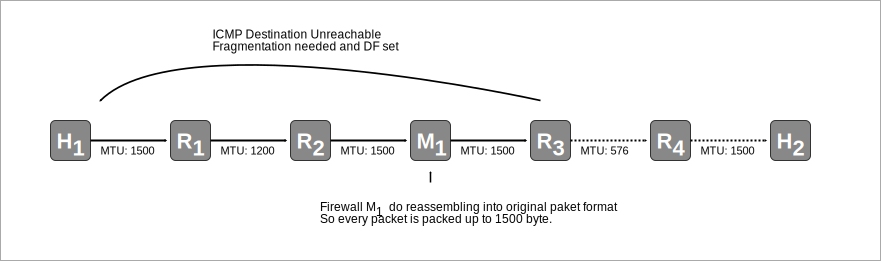
\includegraphics[scale=0.6]{images/blackbox.pdf}}
 \end{picture}
\bi
	\item Fragmentierung und Defragmentierung benötigt zusätzliche Bearbeitungszeit und führt zu höherer Latenz
	\item Fragmentierung verschlechtert das Kontroll/Nutzlast Verhältnis: jedes Fragment bekommt einen eigenen IP Header (dies wirkt sich negativ auf die PER aus).
	\item Fragmentierung bereitet Firewalls, Analyser, ... Probleme.
	\bi
		\item Im Zweifel werden Pakete verworfen wenn die Firewall nicht reassemblieren kann
		\item Wenn die Firewall fragmentiert kann es zu Blackhole Problemen kommen (siehe Beispiel) 
	\ei
	\item Probleme im Zusammenspiel mit Tunneln (z.B. IPIP, Teredo, OpenVPN)
\ei
\end{slide}


%%%%%%%%%%%%%%%%%%%%%%%%%%%%%%
\begin{slide}
\slidetitle{Vielen Dank}{Vielen Dank}
\bi
	\item Viele Dank
\ei
\end{slide}

\end{document}

% vim600: fdm=marker tw=130 sw=4 ts=4 sts=4 ff=unix noet:
